\chapter{Описание практической части}


\section{Инструментарий}

\begin{itemize}
	\item В качестве языка реализации выбран язык программирования Java
	\item В качестве реализации классификаторов используется библиотека libsvm
	\item В качестве реализации мер над строками используется библиотека secondstring
	\item Для сбора данных для обучения и тестирования написан краулер на Python с использованием библиотеки scrapy
	\item В качестве реализации перевода данных для обучения из формата JSON во внутреннее представление используется библиотека json-simple
\end{itemize}


\section{Общая схема работы}

\begin{enumerate}
	\item Из JSON-файла с базой знаний загружаются записи для множества элементарных исходов
	\item Из входного файла считываются текстовые посты для анализа (по одному на каждой строке) Далее для каждого поста:
	\begin{enumerate}
		\item Предобработка множества элементарных исходов и получение подмножества кандидатов
		\item Связывание поста со схемой
		\item Классификация токенов поста в соответствии со схемой
		\item Чистка атрибутов поста
		\item Результат записывается в файл в виде ``токен метка'' 
	\end{enumerate}
\end{enumerate}


\section{Архитектура системы}

Работа программы начинается с класса \textit{Main}.

Класс \textit{DataStore} служит внутренним представлением базы знаний, с помощью метода \textit{init$\_$base} загружаются данные для обучения и множества элементарных исходов.

Класс \textit{BlockSchemeLearner} с помощью метода \textit{sequential$\_$covering} осуществляет предобработку множества элементарных исходов.

Класс \textit{PostExplorer} осуществляет связывание и извлечение нинформации. Метод \textit{results} производит чистку и запись результатов в выходной файл

На рисунке изображена упрощенная диаграмма классов системы\\
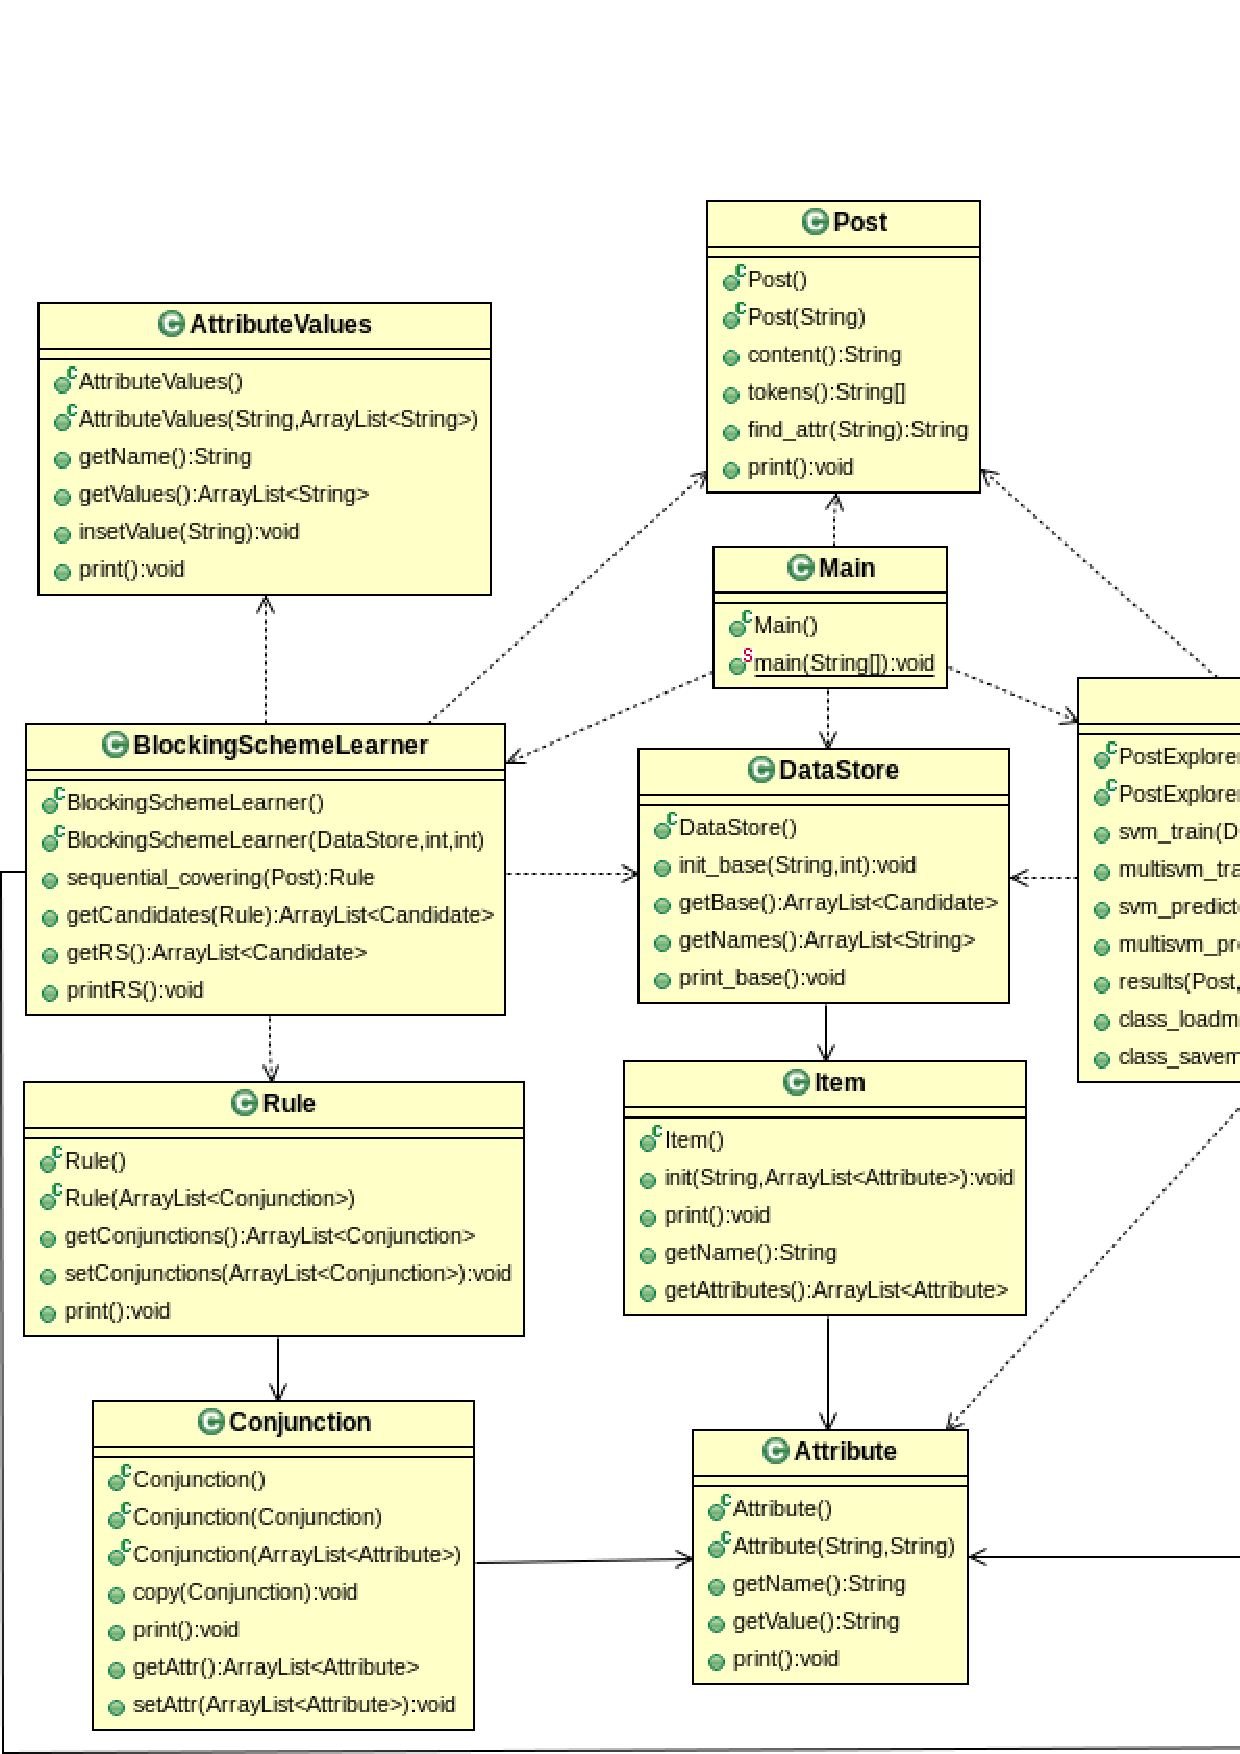
\includegraphics[width=\linewidth]{diagram.png}


\section{Анализ результатов}

Для тестирования работы алгоритма системе была поставлена задача разметки постов о ноутбуках в интернет-магазинах.

Для обучения SVM-классификатора использовались 8055 записей о ноутбуках с сайта amazon.com\footnote{www.amazon.com}. Для обучения Multi-Class SVM-классификатора по 8055 записям были искусственно созданы посты вида $\{\text{значение}\_\text{атрибута}_1 \ldots\text{значение}\_\text{атрибута}_n\}$. Для тестирования использовались 104 вручную размеченные записи о ноутбуках с сайта bestbuy.com\footnote{www.bestbuy.com}

Тестировалось качество разметки поста метками 6 атрибутов: цвет, диагональ экрана, RAM, объем внешней памяти, производитель, линейка

Для оценки качества использовалась $F_1 \text{мера} (\frac{2*Precision*Recall}{Precision + Recall}$). Значение меры вычислялось для каждого атрибута по-отдельности.\\

\begin{table}[H]
\caption{Результаты тестирования.}
\begin{center}
\begin{tabular}{|l|c|c|c|}
\hline
Атрибут & Precision & Recall & $F_1$\\
\hline
Цвет & 0.4462 & 0.7632 & 0.5631\\
Диагональ экрана & 0.9216 & 0.9592 & 0.94\\
RAM & 0.3789 & 0.72 & 0.4966\\
Память & 0.6094 & 0.7959 & 0.6903\\
Производитель & 0.8621 & 1.0 & 0.9259\\
Линейка & 0.2621 & 0.6585 & 0.375\\
\hline
Среднее & 0.58 & 0.8162 & 0.6652\\
\hline
\end{tabular}
\end{center}
\end{table}



В целом результат работы несколько хуже, чем таковой у авторов подхода. Этому может быть 2 причины.

1 причина заключается в неоднородности обучающей выборки Multi-Class SVM-классификатора и сильном разбросе значений атрибутов. Лучшее значение $F_1 \text{меры}$ достигнуто на атрибуте ``диагональ экрана'', этот атрибут есть почти у всех моделей и диапазон его значений довольно узок (около 10). В то время как атрибута ``линейка'' нет почти у половины записей в обучающей выборке, и диапазон значений очень широкий (его ширина сравнима с количеством записей).

2 причина заключается в процедуре чистки атрибутов и косвенно зависит от 1 причины. Из-за того, что в обучающей выборке недостаточно записей, содержащих, например, атрибут ``линейка'', то классификатор токен входного поста, относящийся к атрибуту ``линейка'' с большой вероятностью разметит другим атрибутом. В процессе чистки, таким образом, данный токен в лучшем случае станет ``пустышкой''. Поскольку пороговый минимум в конце чистки определяется исходя из обучающей выборки, а средняя длина значения атрибута ``линейка'' велика (более 15 символов), значения мер в чистке несколько больше, чем должно быть (так как ``мусорных'' токенов в посте обычно мало и они коротки). В результате страдает разметка токенов атрибутами, длина чьих значений очень мала (около 4 символов) - такие токены становятся ``пустышками''. Об этом свидетельствует низкая точность определения атрибута ``RAM''. 